\section{Bi-orthogonal Bases}\label{sec: bi-orth}
In this section, we analyze bi-orthogonal bases in the following form of MRA,
\begin{align}\label{eq: bi-orth MRA}
\{\phi_{L,\V{k}},\widetilde{\phi}_{L,\V{k}}, \psi_{l,\V{k}'}^j,\widetilde{\psi}_{l,\V{k}'}^j,\, 1\leq l\leq L,\,\V{k}\in\mathbb{Z}^2,\, \V{k}'\in\mathbf{Q}\mathbb{Z}^2,\,1\leq j\leq J \},
\end{align}
where $\phi$ and $\psi^j$ satisfy \eqref{eq: m0} and \eqref{eq: mj}, as well as $\widetilde{\phi}$ and $\widetilde{\psi^j}$, respectively,
$$\widehat{\widetilde{\phi}}(\V{D}^T\V{\omega}) = \widetilde{m_0}(\V{\omega})\widehat{\widetilde{\phi}}(\V{\omega}),\quad \widehat{\widetilde{\psi^j}}(\V{D}^T\V{\omega}) = \widetilde{m_j}(\V{\omega})\widehat{\widetilde{\phi}}(\V{\omega}).$$
For such bi-orthogonal bases, we have the similar identity summation and shift cancellation condition to those in Theorem \ref{thm: conds}.
\begin{thm}\label{thm: bi-orth conds}
The perfect reconstruction iff the following two conditions hold
\begin{align}\label{eq: id-sum 2}
m_0(\boldsymbol{\omega})\sbarm{0} + \sum_{j = 1}^6 m_j(\boldsymbol{\omega})\sbarm{j} = 1
\end{align}
\begin{equation}\label{eq: shift-cancel 2}
\begin{cases}
\sum_{j = 0}^6m_j(\boldsymbol{\omega})\overline{\widetilde{m_j}}(\boldsymbol{\omega} + \boldsymbol{\pi}) = 0, & \boldsymbol{\pi}\in \Gamma_0\setminus\{\boldsymbol{0}\}\\[.5em]
\sum_{j=1}^6m_j(\boldsymbol{\omega})\overline{\widetilde{m_j}}(\boldsymbol{\omega}+\boldsymbol{\pi}) = 0, & \boldsymbol{\pi}\in\Gamma_1\setminus\Gamma_0
\end{cases}
\end{equation}
\end{thm}
The conditions \eqref{eq: id-sum 2} and \eqref{eq: shift-cancel 2} can be combined into a linear system as follows,
\begin{align}\label{eq: LS-new}
%\overline{\M}(\V{\omega})\mathbf{m}_0(\V{\omega})=
\begin{bmatrix}
    \,\sbarm{0} & \sbarm{1} & \hdots & \sbarm{6}\;  \\
    \;0 & \sbarmp{1}{1}  & \hdots  & \sbarmp{6}{1}\; \\
    \,\sbarmp{0}{2} & \sbarmp{1}{2} & \hdots & \sbarmp{6}{2}\;\\
    \;\vdots & \vdots & \vdots & \vdots \; \\
    \;0 & \sbarmp{1}{7} & \hdots & \sbarmp{6}{7}\;
\end{bmatrix}
\begin{bmatrix}
\;\mo{0}\; \\
\;\mo{1}\; \\
\;\mo{2}\; \\
\; \vdots\; \\
\;\mo{6}\; 
\end{bmatrix} 
=
\begin{bmatrix}
1\\
0\\
0\\
\vdots \\
0
\end{bmatrix}
\end{align}
%where $\M\in\mathbb{C}^{8\times 7}$ and $\mathbf{m}_0\in\mathbb{C}^7$.
In addition, we have the following analogue of Theorem \ref{thm: basis cond}.
\begin{thm}\label{thm: basis cond 2}
Assume that $m_0, \widetilde{m_0}$ are trigonometric polynomials with $m_0(0)=\widetilde{m_0}(0) = 1$, which generate $\phi,\widetilde{\phi}$ respectively.\\
If $\phi(\cdot - \boldsymbol{k}),\widetilde{\phi}(\cdot - \boldsymbol{k}),\,\boldsymbol{k}\in\mathbb{Z}^2$ are bi-orthogonal, then $\exists K$ containing a neighborhood of 0, s.t. $\forall\boldsymbol{\omega}\in S_0,\,\boldsymbol{\omega}+2\pi\mathbf{n}\in K$ for some $\mathbf{n}\in\mathbb{Z}^2, $ and $\inf_{k>0,\,\boldsymbol{\omega}\in K}|m_0(\mathbf{D_2}^{-k}\boldsymbol{\omega})| >0$, $\inf_{k>0,\,\boldsymbol{\omega}\in K}|\widetilde{m_0}(\mathbf{D_2}^{-k}\boldsymbol{\omega})| >0$. 
 Further, if  $\sum_{\boldsymbol{\V{\pi}}\in \Gamma_0} m_0(\boldsymbol{\omega}+\boldsymbol{\pi})\sbarmp{0}{} = 1,$ then the inverse is true.
\end{thm}
By Theorem \ref{thm: basis cond 2}, $m_0$ and $\widetilde{m_0}$ need to satisfy the following identity constraint for the MRA \eqref{eq: bi-orth MRA} to be bi-orthogonal,
\begin{align}\label{eq: identity-cond}
m_0\sbarm{0} + m_0\sbarmp{0}{2} + m_0\sbarmp{0}{4} + m_0\sbarmp{0}{6} = 1.
\end{align}
In sum, the construction of a bi-orthogonal basis \eqref{eq: bi-orth MRA} is equivalent to find feasible solutions of \eqref{eq: LS-new} with constraint \eqref{eq: identity-cond}. To solve \eqref{eq: LS-new}, we use the same approach in \cite{cohen1993compactly}, which solves compactly supported symmetric bi-orthogonal filters on hexagon lattice. We next review the main scheme in \cite{cohen1993compactly} and extend it to our setup of directional wavelet filter.

\subsection{Summary of Cohen et al's construction}\label{subsec: cohen-summary}
We summerize the main setup and the approach in \cite{cohen1993compactly}. Consider a bi-orthogonal scheme consists of 3 high-pass filters $m_1,m_2$ and $m_3$ and a low-pass filter $m_0$ together with their bi-orthogonal duals $\widetilde{m_j}$, s.t.
$m_0$ is $\frac{2\pi}{3}$-rotation invariant and $m_1,\, m_2,\, m_3$ are $\frac{2\pi}{3}$-rotation co-variant.

This bi-orthogonal scheme satisfies the following linear system (
Lemma 2.2.2 in \cite{cohen1993compactly} )
\begin{align}\label{eq: LS}
\begin{bmatrix}
    \, \overline{\widetilde{m_0}}(\V{\omega}) &  \overline{\widetilde{m_1}}(\V{\omega}) &  \overline{\widetilde{m_2}}(\V{\omega}) &  \overline{\widetilde{m_3}}(\V{\omega})\; \\
    \;\sbarmn{0}{1} & \sbarmn{1}{1}  & \sbarmn{2}{1}  & \sbarmn{3}{1}\; \\
    \;\vdots & \vdots & \vdots & \vdots \; \\
    \;\sbarmn{0}{3} & \sbarmn{1}{3} & \sbarmn{2}{3} & \sbarmn{3}{3}\;
\end{bmatrix}
\begin{bmatrix}
\;\mo{0}\; \\
\;\mo{1}\; \\
\;\mo{2}\; \\
\;\mo{3}\; 
\end{bmatrix} 
=
\begin{bmatrix}
1\\
0\\
0\\
0
\end{bmatrix}
\end{align}
 where $\V{\nu}_1 = (\pi,0),\V{\nu}_2 = (0,\pi),\V{\nu}_3=(\pi,\pi)$.
 Let $\widetilde{\mathbf{M}}(\V{\omega})\in\mathbb{C}^{4\times 4}$ be the matrix with $\barm{j}$ entries and $\mathbf{m}(\V{\omega})\in\mathbb{C}^4$ be the vector with $m_j$ entries in \eqref{eq: LS}, then \eqref{eq: LS} can be written as \(\widetilde{\mathbf{M}}\, \mathbf{m} (\V{\omega})= [1,0,0,0]^\top\).\\
Given $\m{1}$, $\m{2},\,\m{3}$ are determined by symmetry, and Lemma 2.2.2 in \cite{cohen1993compactly} shows that
\begin{align}\label{eq: m0-sol}
m_0(\V{\omega}) &= D^{-1}%\propto 
\left|
\begin{matrix}
    \; \sbarmn{1}{1}  & \sbarmn{2}{1}  & \sbarmn{3}{1}\; \\
    \; \sbarmn{1}{2}  & \sbarmn{2}{2}  & \sbarmn{3}{2}\; \\
    \; \sbarmn{1}{3} & \sbarmn{2}{3} & \sbarmn{3}{3}\;
\end{matrix}
\right| \notag\\
&= D^{-1}\det(\widetilde{\mathbf{M}}_{1,1}(\V{\omega})),
\end{align}
where $ D \equiv \det(\widetilde{\mathbf{M}})\in \mathbb{C}^* = \mathbb{C}\setminus\{0\}$.
%{\it Remark.} 
%For \eqref{eq: m0-sol} to hold, $m_0(\mathbf{\omega})$ and $\det(\widetilde{\mathbf{M}}_{1,1}(\V{\omega}))$ having the same phase suffices, which is implied by the symmetry of $m_0$ and $\widetilde{m_j} $'s.\\ % Both $\mo{0}$ and $\det(\widetilde{\mathbf{M}}_{1,1}(\V{\omega}))$ are $\frac{2\pi}{3}-$rotation invariant. \\
If $\widetilde{m_0}$ is solved, then $m_1,m_2$ and $m_3$ are obtained by solving the linear system \eqref{eq: LS}.
To get $\m{0}$, we solve 
\begin{align}\label{eq: bi-orth-eq}
m_0\sbarm{0} + m_0\sbarmn{0}{1} + m_0\sbarmn{0}{2} + m_0\sbarmn{0}{3} = 1
\end{align}
from expanding $det(\widetilde{\mathbf{M}})$ with respect to the first column.
According to Lemma 3.2.1 in \cite{cohen1993compactly} based on {\it Hilbert's Nullstellensatz}, \eqref{eq: bi-orth-eq} has a solution iff there does not exist $(z_1,z_2)\in (\mathbb{C}^*)^2,\, \mathbb{C}^* = \mathbb{C}\setminus\{0\}$\, s.t. $(\pm z_1,\pm z_2)$ are all 
vanishing points of the $z$-transform of $m_0$.

%\subsubsection{Solving $\m{0}$}
In general, there is no efficient algorithm to solve {\it Hilbert's Nullstellensatz}, and how \eqref{eq: m0-sol} is solved exactly is not mentioned in \cite{cohen1993compactly}.
In the next section, we propose an optimization approach, where \eqref{eq: m0-sol}(which is the same as \eqref{eq: identity-cond}) serves as a linear constraint and the objective function imposes regularity on $\widetilde{m_0}$.


\section{Adaptation to dilated quincunx scheme}

\textcolor{red}{Replace by an overview of this section}

Following the same approach of Cohen et al, we focus on solving $m_i$'s and $\widetilde{m_0}$ in \eqref{eq: LS-new} given pre-designed $\m{i},\,i=1,\cdots,6$. %Assume $\m{i},\,i=1,\cdots,6$ satisfy weak constraints on the direction selectivity of their support.

Since \eqref{eq: LS-new} takes the same form as \eqref{eq: LS}, for simplicity, in the rest of this paper, we reuse matrix and vector notations $\widetilde{\mathbf{M}}(\V{\omega}),\,\mathbf{m}(\V{\omega}) $ in \eqref{eq: LS} for those in \eqref{eq: LS-new}, where $\widetilde{\mathbf{M}}(\V{\omega})\in\mathbb{C}^{8\times 7}$ and $\mathbf{m}(\V{\omega})\in\mathbb{C}^7$. In addition, let $\V{b}_k \in\mathbb{R}^8,\, 0\leq k\leq 7$, whose only non-zero entry is $\V{b}_k[k] = 1$, where the indexing starts with zero. Note that $\M\,\mathbf{m}(\V{\omega}) = \V{b}_0\in\mathbb{R}^8$ is over-determined, and it has unique solution if and only if 
\begin{itemize}
\item[(i)] $\M(\V{\omega})$ is full rank,
\item[(ii)] $[\M(\V{\omega}), \V{b}_0]$ is singular.
\end{itemize}
The matrix $\M(\V{\omega})$ is structured such that each row is associated with a shift $\V{\pi}_i,\,i=0\cdots,7$ and each column is associated with a dual function $\m{j},\,j=0,\cdots,7$. We introduce the following notation on $\M$. We denote a sub-matrix of $\M$ containing all but the row associated with $\V{\pi}_k$(the column associated with $\m{k}$) as $\M[-k,:]$($\M[:,-k]$).
In particular, we denote $\M[-0,-0]$ as $\Msub$.

\begin{lemma}\label{lem: subM-singular}
If \eqref{eq: LS-new} is solvable, then $\M[-0,:](\V{\omega})$ is singular $\forall \V{\omega}$.
\end{lemma}
\noindent{\it Proof.}
If \eqref{eq: LS-new} is solvable, then condition (ii) holds, which implies that $\det([\M,\V{b}_0]) = 0$. Expanding the determinant with respect to the last column $\V{b}_0$ yields $\det(\M[-0,:]) = 0$.\qed\\[1em]
%If \eqref{eq: LS-new} has a solution, then $\forall \V{\omega}$,  $[1,0,\cdots,0]^\top\in \mathbb{R}^8$ is a linear combination of the columns of $\M$ hence the solution $\mathbf{m} \in Null(\M[-0,:])$ and it is non-zero. This implies that $\M[-0,:]$ is singular.\qed\\[1em]
We have the following observation on the symmetry of $\M(\V{\omega})$ due to the $(2\pi,2\pi)$-periodicity of shifts $\V{\pi}_i$'s.
\begin{lemma}\label{lem: M-symmetry}
$\M(\V{\omega}),\,\M(\V{\omega}+\V{\pi}_2),\,\M(\V{\omega}+\V{\pi}_4)$ and $\M(\V{\omega}+\V{\pi}_6)$ are the same up to row permutations. \eqref{eq: LS-new} holds $\forall \, \V{\omega}$ if and only if 
\begin{align*}
\M(\V{\omega}) \big[\,\mathbf{m}(\V{\omega}),\mathbf{m}(\V{\omega}+\V{\pi}_2),\mathbf{m}(\V{\omega}+\V{\pi}_4),\mathbf{m}(\V{\omega}+\V{\pi}_6)\,\big] = \big[\,\V{b}_0,\V{b}_2,\V{b}_4,\V{b}_6\,\big]
\end{align*}
\end{lemma}

Due to condition (i), $\forall\,\V{\omega}$, $\exists\, k_{\V{\omega}}$ such that $\M[-k_{\V{\omega}},:]$ is non-singular. On the other hand, Lemma \ref{lem: subM-singular} and Lemma \ref{lem: M-symmetry} together imply that $\M[-k,:],\,k=0,2,4,6$ are singular. Therefore, $k_{\V{\omega}} \in\{1,3,5,7\}$. 
As in Section \ref{subsec: cohen-summary}, we compute $m_0$ by applying Cramer's rule to $\M[-k_{\V{\omega}},:]$, 
%there is a unique row $\M[k_{\V{\omega}},:],\,k_\omega\in\{2,\cdots,8\}$ such that removing it from $\M$ gives a non-singular square matrix $\M[-k_{\V{\omega}},:]$. By Cramer's rule, 
\begin{align}\label{eq: m0-cramer}
m_0(\V{\omega}) = \det(\Msub[-k_{\V{\omega}},:])/\det(\M[-k_{\V{\omega}},:]).
\end{align}
Moreover, the identity condition \eqref{eq: identity-cond} on $m_0(\V{\omega})$ and $\m{0}$ can be derived in the same way as \eqref{eq: bi-orth-eq} by expanding $\det(\M[-k_{\V{\omega}},:])$.

In the following subsections, we first show our main result that for \eqref{eq: LS-new} to be solvable, the pre-designed $\widetilde{m_i}$'s are discontinuous, when a minimum symmetry of $\m{j}$'s is required. We then discuss how to design $\widetilde{m_i}$'s with more symmetry and solve the corresponding system \eqref{eq: LS-new}.

\subsection{Discontinuity of $\m{i}$}
In this subsection, we assume that
$|\m{1}|$ and $|\m{6}|$ are symmetric with respect to the diagonal $\omega_1=\omega_2$, i.e.
$$ |\widetilde{m_1}(\V{\omega})| = |\widetilde{m_6}(\V{\omega}')|\quad \forall\, \omega_1=\omega_2', \,\omega_2=\omega_1',$$
and likewise for $\m{3}$ and $\m{4}$,
$$ |\widetilde{m_3}(\V{\omega})| = |\widetilde{m_4}(\V{\omega}')|\quad \forall\, \omega_1=-\omega_2', \,\omega_2=-\omega_1'.$$
%Same as in Section \ref{subsec: cohen-summary} , we first compute $m_0$ and assume that $\M$ is full rank, otherwise \eqref{eq: LS-new} has infinitely many solutions. Moreover, $\M[2:8,:]$ is singular. 
Let $\mrow{i}(\V{\omega}) = [\widetilde{m_1}(\V{\omega}+\V{\pi}_i)\, \cdots,\,\widetilde{m_6}(\V{\omega}+\V{\pi}_i)]\in\mathbb{C}^6,\, i = 0,\cdots,7$ be the rows of $\M[:,-0]$, and define $$d_{i,j}(\V{\omega}) = \det([\mrow{k_1}(\V{\omega})^\top,\cdots,\mrow{k_6}(\V{\omega})^\top]),\;$$ where $0\leq k_1<\cdots<k_6\leq 7,\, s.t.\, k_l\neq i,j.$
\begin{lemma}\label{lem: subM-singular-sys}
\eqref{eq: LS-new} is solvable $\forall \V{\omega}$ if and only if \vspace{.5em}
\begin{align}
\label{eq: singular-cond}
\mathfrak{D}(\omega)\begin{bmatrix}
\sbarm{0}\\
\sbarmp{0}{2}\\
\sbarmp{0}{4}\\
\sbarmp{0}{6}
\end{bmatrix}
\doteq
\begin{bmatrix}
0 & d_{0,2} & d_{0,4} & d_{0,6}\\
-d_{0,2} & 0 & d_{2,4} & d_{2,6}\\
-d_{0,4} & -d_{2,4} & 0 & d_{4,6}\\
-d_{0,6} & -d_{2,6} & -d_{4,6} & 0
\end{bmatrix}
\begin{bmatrix}
\sbarm{0}\\
\sbarmp{0}{2}\\
\sbarmp{0}{4}\\
\sbarmp{0}{6}
\end{bmatrix}
= \begin{bmatrix}
0\\0\\0\\0
\end{bmatrix}.
\end{align}
\end{lemma}
\noindent{\it Proof.}
By Lemma \ref{lem: subM-singular} and Lemma \ref{lem: M-symmetry},  $\M[-k,:],\,k=0,2,4,6$ are singular,
The singularity condition on  $\M[-0,:](\V{\omega})$ can be rewritten as follows,
\begin{align}\label{eq: singular-omega}
0 &=\det(\M[-0,:]) \notag\\
&=  \sbarmp{0}{2}\cdot\det(\Msub[-2,:])\notag\\
&\quad+ \,\sbarmp{0}{4}\cdot\det(\Msub[-4,:])
+ \sbarmp{0}{6}\cdot\det(\Msub[-6,:])\notag\\
&= 0\cdot\sbarm{0}\,+\,d_{0,2}\cdot\sbarmp{0}{2} \notag\\
&\quad+\,d_{0,4}\cdot \sbarmp{0}{4}\,+\, d_{0,6}\cdot\sbarmp{0}{6}
\end{align}
%This is the first equation in the linear system \eqref{eq: singular-cond}. Substitute $\V{\omega}$ by $\V{\omega + \pi_2}$ in \eqref{eq: singular-omega} and use the $2\pi-$periodicity of $\V{\omega}$, we have the singularity condition on $\M[-1,:](\V{\omega+\pi_2})$ as follows
%then the above singularity condition on $\M[-1,:]$ at $\V{\omega}$ can be rewritten as follows,
%\begin{align*}
%[0,\, d_{0,2}(\V{\omega}),\, d_{0,4}(\V{\omega}),\, d_{0,6}(\V{\omega})]\,[\widetilde{m_0}(\V{\omega}),\,\widetilde{m_0}(\V{\omega}+\V{\pi}_2),\, \widetilde{m_0}(\V{\omega}+\V{\pi}_4),\,\widetilde{m_0}(\V{\omega}+\V{\pi}_6)]^\top = 0
%\end{align*}
%It is easy to verify that the above singular condition at $\V{\omega}+\V{\pi}_2$ is equivalent to 
%\begin{align*}
%-d_{0,2}(\V{\omega})\cdot \widetilde{m_0}(\V{\omega}) + d_{2,4}(\V{\omega})\cdot \widetilde{m_0}(\V{\omega}+\V{\pi}_4) + d_{2,6}(\V{\omega})\cdot\widetilde{m_0}(\V{\omega}+\V{\pi}_6) = 0,
%[-d_{0,2}(\V{\omega}),\, 0,\,d_{2,4}(\V{\omega}),\,d_{2,6}][\widetilde{m_0}(\V{\omega}),\,\widetilde{m_0}(\V{\omega}+\V{\pi}_2),\, \widetilde{m_0}(\V{\omega}+\V{\pi}_4),\,\widetilde{m_0}(\V{\omega}+\V{\pi}_6)]^\top = 0,
%\end{align*}
%which is the second linear equation in  \eqref{eq: singular-cond}.
Similarly, the second to fourth equations can be obtained by rewriting the singularity condition on $\M[-2,:]$, $\M[-4,:]$ and $\M[-6,:]$ respectively.\qed
% at $\V{\omega}+\V{\pi}_4$ and $\V{\omega}+\V{\pi}_6$ in the coordinate of $\V{\omega}$.\qed
%where $\mathfrak{D}(\V{\omega})$ is anti-symmetric. Because $\mathfrak{D}(\V{\omega})$ is independent of $m_0(\V{\omega})$, \eqref{eq: singular-cond} holds for $\mc{0}$ as well.

%On the other hand, given $m_0$, $\widetilde{m_0}$ has to satisfy the identity constraint \eqref{eq: identity-cond}.
The identity constraint \eqref{eq: identity-cond} on $m_0$ and the singularity condition \eqref{eq: singular-cond} together imply the following proposition,
%Due to the periodic wrapping of the frequency square $S_0$, we only need to consider \eqref{eq: singular-cond} and \eqref{eq: identity-cond} on $S_1$ and they imply the following proposition,
\begin{proposition}\label{prop: feasibility}
Given $\widetilde{m_i}, i = 1,\cdots,6$, \eqref{eq: LS-new} has no solution for $\widetilde{m_0}$, if $\exists\,\omega, \,s.t. \; [m_0(\omega), m_0(\omega+\pi_2),m_0(\omega+\pi_4),m_0(\omega+\pi_6)]$ is a linear combination of the rows of $\mathfrak{D}(\omega)$.% in \eqref{eq: singular-cond}.
\end{proposition}
%Proposition \ref{prop: feasibility} provides a necessary condition such that the numerical optimization solving $\widetilde{m_0}$ is feasible.
\begin{figure}
\centering
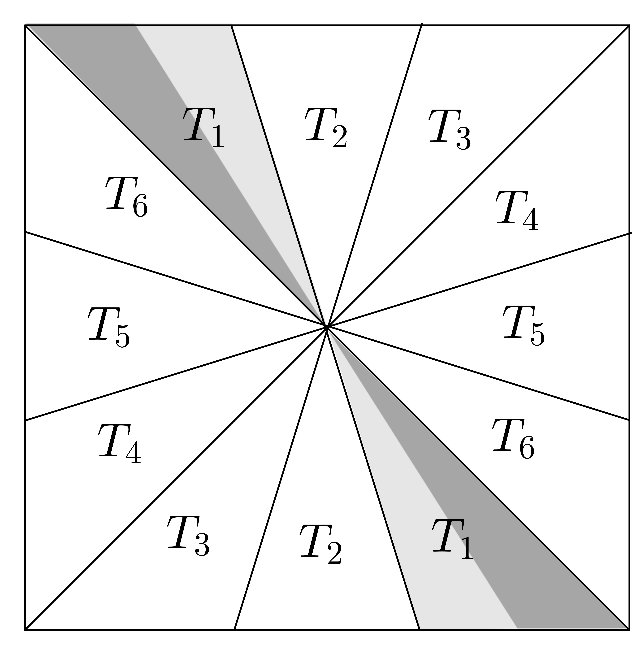
\includegraphics[width = .4\textwidth]{triangle-partition-new.png}
\caption{Partition of frequency square in six directions, where the essential support of $\m{i}$ is contained in each pair of triangles $T_i$. The pair of dark grey triangles is $T_1^-$ and the light grey pair is $T_1^+$.}
\label{fig: partition 2}
\end{figure}
%Let pairs of triangles $T_i$ in Fig.\ref{fig: partition 2} contain the essential support of $\widetilde{m_i},\,i=1,\cdots,6$.
%\eqref{eq: LS-new} takes a similar form to \eqref{eq: LS}, but with $\M\in\mathbb{C}^{8\times 7}$, which is an over-determinant linear system.

\noindent{\bf Definition.}
The {\it essential support} $\Omega_i$ of a function $\widetilde{m_i}$ is the set $\{\V{\omega}:\,|\widetilde{m_i}(\V{\omega})|> |\widetilde{m_j}(\V{\omega})|,\,\forall j\neq i\}$. \vspace{.5em}

Let $T_i$ be pairs of triangles shown in Figure \ref{fig: partition 2}, such that $C_i\subset T_i,\, i = 1,\cdots,6.$ Consider its decomposition, $T_i = T_i^-\bigcup T_i^+$, where $T_i^-, T_i^+$ are halves of $T_i$ adjacent  to $T_{i-1}$ and $T_{i+1}$ respectively.\\[.5em]
\noindent{\bf Definition.}  $\widetilde{m_i}$ {\it concentrates} within cone $T_i$ if 
\begin{itemize}
\item[(i)] $\Omega_i\subset T_i$;
\item[(ii)]$\text{supp}(\widetilde{m_i})\subset T_{i-1}^+\bigcup T_i\bigcup T_{i+1}^-$ and $\int_\Omega|\widetilde{m_i}| > \int_{\Omega'}|\widetilde{m_i}|, \forall\, \Omega\subset T_i\bigcap\text{supp}(\widetilde{m_i})$, where $\Omega' \subset T_{i-1}^+\bigcup T_{i+1}^-$ is symmetric to $\Omega$ with respect to the boundary of $T_i$.
\end{itemize}

\begin{figure}
\centering
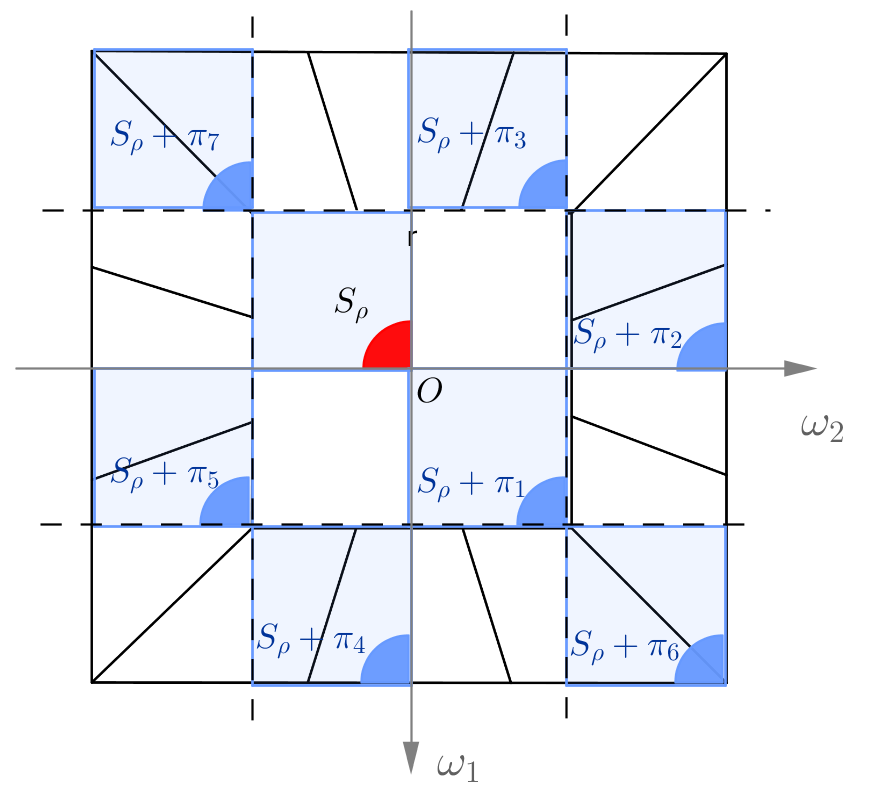
\includegraphics[width = .5\textwidth]{S_shifts2.png}
\caption{$S_{\rho}$ and its shifts}
\label{fig: S-shifts}
\end{figure}
Given $\m{i}$ that concentrates in $T_i$, we study the feasibility condition in Proposition \ref{prop: feasibility} specifically on the domain $S_{\rho} = \{(\omega_1,\omega_2)|\;\Vert\omega\Vert < \rho, \omega_1 <0,\,\omega_2<0\}$, see Figure \ref{fig: S-shifts}. 

\begin{lemma}\label{lem: rank1}
$\exists\, \rho>0$ s.t. $\forall \omega\in S_\rho$, $rank(\mrow{1},\mrow{7})=1$ or $rank(\mrow{3},\mrow{5}) = 1$.
\end{lemma}
\noindent{\it Proof.}
When $\rho$ is small enough, due to the concentration property, $\m{i}$ is zero on all but a few sets $S_\rho + \V{\pi}_j$ (see Fig.\ref{fig: S-shifts} for reference of $S_\rho$ and its shifts), thus $\mrow{i}(\V{\omega})$ is sparse on $S_\rho$ and $\M[-0,:]$ takes the following form
\begin{align}
\label{eq: sparse-mat}
\M[-0,:](\V{\omega})=
\begin{bmatrix}
\mrow{0}\\
\mrow{1}\\
\mrow{2}\\
\mrow{3}\\
\mrow{4}\\
\mrow{5}\\
\mrow{6}\\
\mrow{7}
\end{bmatrix}
=
\begin{bmatrix}
0 & 0 & 0 & 0 & 0 & 0\\
* & 0 & 0 & 0 & 0 & *\\
0 & 0 & 0 & * & * & 0\\
0 & 0 & * & * & 0 & 0\\
0 & * & * & 0 & 0 & 0\\
0 & 0 & * & * & 0 & 0\\
* & 0 & * & * & 0 & *\\
%0 & * & * & 0 & 0 & 0\\
%0 & 0 & 0 & * & * & 0\\
%* & 0 & 0 & 0 & 0 & *\\
%* & 0 & 0 & 0 & 0 & *\\
%0 & 0 & * & * & 0 & 0\\
%0 & 0 & * & * & 0 & 0\\
* & 0 & 0 & 0 & 0 & *
\end{bmatrix}
%=\V{P}\,\widetilde{\mathbf{M}}[:,2:7],
\end{align}
where $*$s denote possible non-zero entries.
%where $\V{P}$ is a row permutation matrix. 
We make the following observation of $\mrow{i}$:
\begin{itemize}
\item[(i)] $\mrow{0}$ is a zero vector
\item[(ii)] $\mrow{2}$ and $\mrow{4}$ are linearly independent of each other and the rest of $\mrow{i}$
\item[(iii)] $span\{\mrow{1},\mrow{7}\} \perp span\{\mrow{3},\mrow{5}\}$ and $rank(\mrow{1},\mrow{7}) \leq 2$, \\$rank(\mrow{3},\mrow{5})\leq 2$
\item[(iv)] $span\{\mrow{1}, \mrow{7}, \mrow{3},\mrow{5},\mrow{6}\} \leq 4$
\end{itemize}
Since $S_\rho$ is in the low frequency domain, $m_0(\V{\omega})\neq 0$. \eqref{eq: m0-cramer} then implies that $\Msub$ is full rank, or equivantly, $rank(\M[-0,:]) = 6$. It follows from  (ii) and (iv) that $rank(\mrow{1},\mrow{6},\mrow{7},\mrow{3},\mrow{5})= 4$.\\
On the other hand, (ii) and (iv) imply that $$rank(\Msub(\V{\omega}+\V{\pi}_2))=rank(\mrow{0},\mrow{4},\mrow{6},\mrow{1},\mrow{3},\mrow{5},\mrow{7})= 5$$ and likewise $$rank(\Msub(\V{\omega}+\V{\pi}_4))=rank(\mrow{0},\mrow{2},\mrow{6},\mrow{1},\mrow{3},\mrow{5},\mrow{7})= 5.$$ Therefore, $\det(\Msub(\V{\omega} + \V{\pi}_2)) = \det(\Msub(\V{\omega} + \V{\pi}_4)) = 0$ and \eqref{eq: m0-cramer} implies $m_0(\V{\omega}+\V{\pi}_2) = m_0(\V{\omega}+\V{\pi}_4) = 0$.\\
If $\mrow{1}$ and $\mrow{7}$ are linearly independent and so are $\mrow{3}$ and $\mrow{5}$, then $$rank(\Msub(\V{\omega}+\V{\pi}_6))=rank(\mrow{2},\mrow{4},\mrow{1},\mrow{3},\mrow{5},\mrow{7}) = 6,$$ hence $m_0(\V{\omega}+\V{\pi}_6)\neq 0$. Therefore, $$[m_0(\V{\omega}),m_0(\V{\omega}+\V{\pi}_2),m_0(\V{\omega}+\V{\pi}_4),m_0(\V{\omega}+\V{\pi}_6)] = [*,0,0,*].$$ In addition, $d_{i,j} = 0,\, \forall(i,j)$ except $(0,6)$, so in \eqref{eq: singular-cond} $$\mathfrak{D}(\V{\omega}) = [d_{0,6}, 0, 0,0]^\top [0,0,0,1] + [0,0,0,d_{0,6}]^\top [-1,0,0,0].$$  By Proposition \ref{prop: feasibility}, the linear system \eqref{eq: LS-new} has no solution $\widetilde{m_0}$ and this proofs the lemma.\qed\\[.5em]
Without loss of generality, in the following analysis, we assume $rank(\mrow{1},\mrow{7}) = 1$ on $S_\rho$.
\begin{lemma}\label{lem: concentrate}
If $\m{1} (\m{6})$ concentrates in $T_1 (T_6)$, then $|\m{6}| > |\m{1}|\,$ a.e. on $T_6\bigcap \text{supp}(\widetilde{m_6})$ ($|\m{1}| > |\m{6}|$ 
a.e. on $T_1\bigcap\text{supp}(\widetilde{m_1})$).
\end{lemma}
\noindent{\it Proof}
Let $B_6=\{\V{\omega}: |\m{6}| \leq |\m{1}|\}\bigcap T_6\bigcap supp(\widetilde{m_1})$ and $B_1$ be its mirror set with respect to $\omega_1 = \omega_2$ and suppose $|B_6|>0$, then $\int_{B_6}|\m{6}|\leq \int_{B_6}|\m{1}|$. On the other hand, since $\m{1}$ concentrates in $T_1$, we know $\int_{B_1}|\m{1}| > \int_{B_6}|\m{1}|$. Moreover, due to the symmetry of $\m{1},\m{6}$ and $B_1,B_6$, $\int_{B_1}|\m{1}| = \int_{B_6}|\m{6}|$, hence $\int_{B_6}|\m{1}| \geq\int_{B_6}|\m{6}| = \int_{B_1}|\m{1}| $ which results in contradiction.\qed

\begin{proposition}
If  $m_1\,(m_6)$ concentrates within $T_1\,(T_6)$, then $\m{1} = \m{6} = 0,\, a.e. $ on $ S_\rho + \V{\pi}_1$.
\end{proposition}
\noindent{\it Proof.}
Consider frequency domain $S_\rho' = S_\rho\bigcap\{\omega_1<\omega_2\}.$ By Lemma \ref{lem: rank1}, $\exists\,\alpha_{\V{\omega}}\in\mathbb{C}, s.t.\,\mrow{1}(\V{\omega}) = \alpha_{\V{\omega}}\,\mrow{7}(\V{\omega}),\, \forall\, \V{\omega}\in S_\rho',$ i.e. $\widetilde{m_1}(\V{\omega} + \V{\pi}_1) = \alpha_{\V{\omega}}\cdot\widetilde{m_1}(\V{\omega} + \V{\pi}_7)$ and $\widetilde{m_6}(\V{\omega} + \V{\pi}_1) = \alpha_{\V{\omega}}\cdot\widetilde{m_6}(\V{\omega} + \V{\pi}_7)$. On the other hand, Lemma \ref{lem: concentrate} implies that $|\widetilde{m_1}(\V{\omega} + \V{\pi}_7)| \geq |\widetilde{m_6}(\V{\omega} + \V{\pi}_7)|$, hence $|\widetilde{m_1}(\V{\omega} + \V{\pi}_1)| \geq |\widetilde{m_6}(\V{\omega} + \V{\pi}_1)|$. Let $\Omega_6':= (S_\rho+\pi_1)\bigcap T_6$, then $\int_{\Omega_6'}|\m{1}| \geq\int_{\Omega_6'}|\m{6}|$, which will contradict Lemma \ref{lem: concentrate} unless $|\Omega_6'\bigcap\text{supp}(\widetilde{m_6})| = 0$, or equivalently $\alpha_{\V{\omega}}=0$ and so $\m{6} = \m{1} = 0,\,a.e.$ on $\Omega_6'$. By symmetry, $\m{6}=\m{1} = 0,\,a.e. $ on $(S_\rho+\V{\pi}_1)\setminus \Omega_6'$ as well.\qed

\begin{proposition}
$\m{1},\m{6}$ are not continuous at both $(\frac{\pi}{2},\frac{\pi}{2})$ and $(-\frac{\pi}{2},-\frac{\pi}{2})$.
\end{proposition}
\noindent{\it Proof}
If $\m{1}$ is continuous at $(\frac{\pi}{2},\frac{\pi}{2})$, then $\widetilde{m_1}(\frac{\pi}{2},\frac{\pi}{2}) = \lim_{\alpha\rightarrow 1^-}\widetilde{m_1}(\V{\omega}(\alpha)) = 0$, where $\{\V{\omega}(\alpha),\,0\leq \alpha<1\} \subset S_\rho + \V{\pi}_1$ and $\V{\omega}(1) = (\frac{\pi}{2},\frac{\pi}{2})$. By symmetry, we have $\widetilde{m_6}(\frac{\pi}{2},\frac{\pi}{2}) = 0$. Similarly, the continuity at $(-\frac{\pi}{2},-\frac{\pi}{2})$ implies $\widetilde{m_1}(-\frac{\pi}{2},-\frac{\pi}{2}) = \widetilde{m_6}(-\frac{\pi}{2},-\frac{\pi}{2}) = 0$. Therefore $\mrow{1}(0) = \mrow{7}(0) = \mathbf{0}$ which results in contradiction with Lemma \ref{lem: rank1}.\qed\\[1em]%and from \eqref{eq: m0C} $m_0^C(0)=0$ so that $m_0(0)=0$, %  On the other hand, Proposition\ref{prop: origin-det} implies that $m_0(0) = 0$ as $a = |\widetilde{m_1}(\pi_1)| = 0$, which results in contradiction.
The following theorem summarizes our main result.
\begin{theorem}\label{thm: thm}
If  $\m{i}$ concentrates in $T_i$ and $\m{1},\m{6}$ are symmetric to each other,  then  \eqref{eq: LS-new} doesn't have feasible solution given continuous $\m{1}$ and $\m{6}$.
\end{theorem}

\subsection{Design of input $\m{j}$}\label{sec: phase-design}
In this sub-section, we construct $\m{j},\, j = 1,\cdots,6,$ which concentrate in $T_i$ with high symmetry.
Specifically, following the orthonormal construction in \cite{yin2014orthshear}, we consider $\m{j}$ in the form 
\begin{align}\label{eq: m-form}
\m{j} = e^{-i\V{\eta}_j^\top\V{\omega}}|\m{j}|,\quad j = 1,\cdots,6
\end{align}
 where $|\m{j}|$'s have symmetries with respect to the two diagonals and the two axis. Figure \ref{fig: tm_i_m_0} shows such a design of $|\m{j}|$ in the left.
 
Given the symmetries of $\m{j}$, for $|m_0(\V{\omega})| > 0,\, \forall\, |\V{\omega}| < \rho$, $\V{\eta}_j$ have to satisfy certain constraints.
% We want to design the phase $\V{\eta}_k$ such that $m_0(\V{\omega}) > 0, \; \forall \omega\in S_1$. This is the same as requiring $\Msub$ to be full rank. We first show the necessary conditions on phases $\V{\eta}$ of the full rank requirement on $\Msub$.
 
\begin{lemma}\label{lem: phase-ineq}
If $\exists\,\V{\omega}\in D_1:=\{\omega_1=\omega_2,\,\omega_1\in(-\frac{\pi}{2},0)\},\,s.t. \,m_0(\V{\omega})>0,$ then $(\V{\eta}_1-\V{\eta}_6)^\top (\V{\pi}_6-\V{\pi}_7)\neq 0(\text{mod}\,2\pi)$. 
\end{lemma} 
\noindent {\it Proof.}
As $\m{1}$ and $\m{6}$ concentrate in $T_1$ and $T_6$ respectively, $\widetilde{m_1}(\V{\omega} + \V{\pi}_i) = 0$ and  $\widetilde{m_6}(\V{\omega} + \V{\pi}_i) = 0$, $i = 1,\cdots, 5$. Due to symmetry, $|\widetilde{m_1}(\V{\omega})| = |\widetilde{m_6}(\V{\omega})|$ on $\{\omega_1=\omega_2\}$. Let $A = |\widetilde{m_1}(\V{\omega}+\V{\pi}_7)| = |\widetilde{m_6}(\V{\omega}+\V{\pi}_7)|$ and $B=|\widetilde{m_1}(\V{\omega}+\V{\pi}_6)| = |\widetilde{m_6}(\V{\omega}+\V{\pi}_6)|$, then the first and the last columns of $\Msub$ are
  \begin{align*}
  \Msub[:,1] = 
 \begin{bmatrix}
 0\\
 \vdots\\
 0\\
 Ae^{i\V{\eta}_1^\top(\V{\omega}+\V{\pi}_6)}\\
 Be^{i\V{\eta}_1^\top(\V{\omega}+\V{\pi}_7)}
 \end{bmatrix}
 \quad\text{and}\quad
  \Msub[:,6] = 
 \begin{bmatrix}
 0\\
 \vdots\\
 0\\
 Ae^{i\V{\eta}_6^\top(\V{\omega}+\V{\pi}_6)}\\
 Be^{i\V{\eta}_6^\top(\V{\omega}+\V{\pi}_7)}
 \end{bmatrix} .
\end{align*}   
By \eqref{eq: m0-cramer}, if $m_0(\V{\omega})>0, \,\V{\omega}\in D_1$ then $\Msub(\V{\omega})$ is full rank, hence its columns are linearly independent.
In particular, $\Msub[:,1]$ and $\Msub[:,6]$ are linearly independent, which implies that $e^{i(\V{\eta}_1^\top\V{\pi}_6 + \V{\eta}_6^\top\V{\pi}_7)}\neq e^{i(\V{\eta}_6^\top\V{\pi}_6 + \V{\eta}_1^\top\V{\pi}_7)}$%$e^{i(\V{\eta}_1-\V{\eta}_6)^\top(\V{\omega}+\V{\pi}_6)}\neq e^{i(\V{\eta}_1-\V{\eta}_6)^\top(\V{\omega}+\V{\pi}_7)}$ 
 or equivalently $(\V{\eta}_1-\V{\eta}_6)^\top(\V{\pi}_6-\V{\pi}_7)\neq 0(\text{mod}2\pi)$. \qed\\

Similarly, if $\exists\,\V{\omega}\in \{\omega_1 = \omega_2,\, \omega_1\in(0,\frac{\pi}{2})\},\, s.t.\, m_0(\V{\omega}) > 0$, then $(\V{\eta}_1-\V{\eta}_6)^\top (\V{\pi}_6-\V{\pi}_1)\neq 0(\text{mod}\,2\pi)$. These two conditions are equivalent to 
\begin{align*}
(\V{\eta}_1-\V{\eta}_6)^\top(\pi/2,\pi/2)\neq 0 (\text{mod}\,2\pi)\tag{\bf c1.1}
\end{align*}
given that $\V{\eta}_1$ and $\V{\eta}_6$ are integer phases in $\mathbb{Z}^2$.
Considering the other diagonal segment $\{\omega_2 = -\omega_1, |\omega_1| <\frac{\pi}{2}\}$, we have 
\begin{align*}
(\V{\eta}_3-\V{\eta}_4)^\top(-\pi/2,\pi/2)\neq 0 (\text{mod}\, 2\pi)\tag{\bf c1.2}
\end{align*}
%from the full rank condition.

Next, we investigate $\Msub(\V{\omega})$ at the origin.
\begin{proposition}\label{prop: origin-det}
%If $|\widetilde{m_1}(\V{\pi}_1)| = |\widetilde{m_1}(\V{\pi}_7)| = |\widetilde{m_3}(\V{\pi}_3)| = |\widetilde{m_3}(\V{\pi}_5)|$ and $|\widetilde{m_1}(\V{\pi}_6)|= | \widetilde{m_3}(\V{\pi}_6)|$, then 
$\V{\pi}_1^\top(\V{\eta}_1-\V{\eta}_6)\neq \pi(\text{mod}\,2\pi)$ or $\V{\pi}_3^\top(\V{\eta}_3-\V{\eta}_4)\neq \pi(\text{mod}\,2\pi)$. 
\end{proposition}
\noindent{\it Proof.}
%$\Msub(\V{0})$ takes the following form
%$$\begin{bmatrix}
%* & 0 & 0 & 0 & 0 & *\\
%0 & * & 0 & 0 & 0 & 0\\
%0 & 0 & * & * & 0 & 0\\
%0 & 0 & 0 & 0 & * & 0\\
%0 & 0 & * & * & 0 & 0\\
%* & 0 & * & * & 0 & *\\
%* & 0 & 0 & 0 & 0 & *
%\end{bmatrix}$$
%The second and the fifth columns of $\Msub$ have single non-zero entry, $\widetilde{m_2}(\V{\pi}_2)$ and $\widetilde{m_5}(\V{\pi}_4)$ respectively, and are orthogonal to all the rest columns, hence the full-rank constraint of $\Msub$ is reduced to the full-rank constraint on its sub-matrix (with permutation of rows and columns)
 Since $\widetilde{m_0}(\V{0})\neq 0$, as shown in Lemma \ref{lem: rank1}, $rank(\mrow{1},\mrow{6},\mrow{7},\mrow{3},\mrow{5})= 4$ at $\V{\omega} = \V{0}$. This is equivalent to the matrix $\V{A}$ defined in \eqref{eq: matrix-B} to be full rank.
\begin{align}\label{eq: matrix-B}
%\mbox{\V{A}\strut}=
\V{A} = 
\begin{bmatrix}
& & & \\[-1em]
\widetilde{m_1}(\V{\pi}_6) & \widetilde{m_6}(\V{\pi}_6) & \widetilde{m_3}(\V{\pi}_6) & \widetilde{m_4}(\V{\pi}_6) \\
\widetilde{m_1}(\V{\pi}_1) & \widetilde{m_6}(\V{\pi}_1) & 0 & 0\\
\widetilde{m_1}(\V{\pi}_7) & \widetilde{m_6}(\V{\pi}_7) & 0 & 0\\
0 & 0 & \widetilde{m_3}(\V{\pi}_3) & \widetilde{m_4}(\V{\pi}_3)\\
0 & 0 & \widetilde{m_3}(\V{\pi}_5) & \widetilde{m_4}(\V{\pi}_5)\\
\end{bmatrix}
\end{align}
Let $|\widetilde{m_1}(\V{\pi}_1)| = a, \, |\widetilde{m_1}(\V{\pi}_6)|=b$. Due to the symmetry of $\m{j}$,
$|\widetilde{m_1}(\V{\pi}_1)| = |\widetilde{m_1}(\V{\pi}_7)| = |\widetilde{m_6}(\V{\pi}_1)| = |\widetilde{m_6}(\V{\pi}_7)| = |\widetilde{m_3}(\V{\pi}_3)| = |\widetilde{m_3}(\V{\pi}_5)| = |\widetilde{m_4}(\V{\pi}_3)| = |\widetilde{m_4}(\V{\pi}_5)|$ and $|\widetilde{m_1}(\V{\pi}_6)|=| \widetilde{m_6}(\V{\pi}_6)|= | \widetilde{m_3}(\V{\pi}_6)|=| \widetilde{m_4}(\V{\pi}_6)|$. Rewrite $\V{A}$ as follows,
$$\V{A}=
\begin{bmatrix}
b e^{-i\V{\pi}_6^\top\V{\eta}_1} & b e^{-i\V{\pi}_6^\top\V{\eta}_6} & b e^{-i\V{\pi}_6^\top\V{\eta}_3} & b e^{-i\V{\pi}_6^\top\V{\eta}_4}\\
a e^{-i\V{\pi}_1^\top\V{\eta}_1} & a e^{-i\V{\pi}_1^\top\V{\eta}_6} & 0						& 0 \\
a e^{i\V{\pi}_1^\top\V{\eta}_1} & a e^{i\V{\pi}_1^\top\V{\eta}_6} & 0						& 0 \\
0 					& 0 					& a e^{-i\V{\pi}_3^\top\V{\eta}_3} & a e^{-i\V{\pi}_3^\top\V{\eta}_4}\\
0 					& 0 					& a e^{i\V{\pi}_3^\top\V{\eta}_3} & a e^{i\V{\pi}_3^\top\V{\eta}_4}\\
\end{bmatrix}
$$
The product of singular values of $\V{A}$ is 
\begin{align}\label{eq: detB}
\sqrt{\text{det}(\V{A}^* \V{A})} = 4a^3\sqrt{a^2 K_1^2K_2^2 + b^2(Q_1K_2^2 + Q_2K_1^2)},
\end{align}
where $ Q_1 = 1 - \cos(\V{\pi}_6^\top(\V{\eta}_1-\V{\eta}_6))\cos(\V{\pi}_1^\top(\V{\eta}_1-\V{\eta}_6)), Q_2 = 1 - \cos(\V{\pi}_6^\top(\V{\eta}_3-\V{\eta}_4))\cos(\V{\pi}_3^\top(\V{\eta}_3-\V{\eta}_4)), K_1 = \sin(\V{\pi}_1^\top(\V{\eta}_1-\V{\eta}_6)), K_2 = \sin(\V{\pi}_3^\top(\V{\eta}_3-\V{\eta}_4)).$ If $\V{\pi}_1^\top(\V{\eta}_1-\V{\eta}_6) = \V{\pi}_3^\top(\V{\eta}_3-\V{\eta}_4) = \pi (mod\, 2\pi)$, then $K_1 = K_2 = 0$ and $\V{A}$ becomes singular.\qed\\[.5em]
{\it Remark.} In Lemma \ref{lem: phase-ineq}, $\Msub[:,1]$ and $\Msub[:,6]$ being independent only guarantees $\det(\Msub[-k_{\V{\omega}},:])\neq 0$. However, \eqref{eq: m0-cramer} implies that $|m_0(\V{\omega})|\propto \det(\Msub[-k_{\V{\omega}},:])$ hence it is preferred to maximize the determinant. Since
\begin{align*}
\det(\Msub[-k_{\V{\omega}}, :]) = \det\big(\big[\, \Msub[-k_{\V{\omega}},-6], \;\Msub[-k_{\V{\omega}},6] + c \cdot\Msub[-k_{\V{\omega}},1]  \,\big]\big),\quad 
\end{align*}
$\forall c\in \mathbb{C}$, the angle between $\Msub[:,1]$ and $\Msub[:,6]$ should be maximized.
Therefore, a stronger condition than ({\bf c1.1}) is to require $\Msub[:,1]$ and $\Msub[:,6]$ be orthogonal, which is equivalent to 
\begin{align*}
(\V{\eta}_1-\V{\eta}_6)^\top(\pi/2, \pi/2) = \pi \,(\text{mod}\, 2\pi).\tag{\bf c2.1}
\end{align*}
The stronger condition corresponding to ({\bf c1.2}) is 
\begin{align*}
(\V{\eta}_3-\V{\eta}_4)^\top(-\pi/2,\pi/2)=\pi(\text{mod},\,2\pi).\tag{\bf c2.2}
\end{align*} %from the stronger orthogonal condition.

%{\it Remark}
%f $|\m{1}| = |\m{2}|$ on $\{\omega_y = 3\omega_x,\,|\omega_x| > \frac{\pi}{2}\}$ and $m_0(\V{\omega}) > 0$ on $\{\omega_y = 3\omega_x\pm \pi,\,|\omega_y| <\frac{\pi}{2}\}$, then the same conditions ({\bf c1}) and ({\bf c2}) can be derived from full rank and orthogonal conditions respectively for tuples $(\,\V{\eta}_1,\,\V{\eta}_2,(-\pi/2,\pi/2)\,),\,(\,\V{\eta}_2,\V{\eta}_3,(\pi/2,\pi/2)\,),\,(\V{\eta}_4,\V{\eta}_5,\,(\pi/2,\pi/2)\,)$ and $(\,\V{\eta}_5,\V{\eta}_6,\,(-\pi/2,\pi/2)\,)$. 

% If the previous strong orthogonal condition on $\V{\eta}_1, \V{\eta}_3, \V{\eta}_4,\V{\eta}_6$ holds, then $K_1 = K_2 = 0$ and $m_0(0)=m_0^C(0)= 0$. Therefore, the strong orthogonal conditions ({\bf c2}) cannot be satisfied at the same time. 
%In particular, we consider the following constraints on phase $\V{\eta}_k\in \mathbb{Z}^2,\, k = 1,\cdots,6$:
Unfortunately, Proposition \ref{prop: origin-det} prevents ({\bf c2.1}) and ({\bf c2.2}) from holding simultaneously.
We propose the following set of phases
\begin{align}\label{eq: phase-sol}
\V{\eta}_1 = (0,0),\; \V{\eta}_2 = (-1,1),\; \V{\eta}_3 = (0,2),\notag\\
\V{\eta}_4 = (1,0),\; \V{\eta}_5 = (0,-1),\; \V{\eta}_6 = (0,1).
\end{align}
where
\begin{align*}
%\label{eq: phase-constraint}
%&(\V{\eta}_1-\V{\eta}_2)^\top(-\pi/2, \pi/2) = (\V{\eta}_5-\V{\eta}_6)^\top(-\pi/2,\pi/2) = \pi\, (\text{mod}\, 2\pi)\notag\\
%&(\V{\eta}_2-\V{\eta}_3)^\top(\pi/2,\pi/2) = (\V{\eta}_4-\V{\eta}_5)^\top(\pi/2,\pi/2) = \pi\, (\text{mod}\, 2\pi)\\
%&
(\V{\eta}_3-\V{\eta}_4)^\top(-\pi/2, \pi/2) &=-\pi/2\,(\text{mod}\,2\pi)\notag\\
 (\V{\eta}_6 - \V{\eta}_1)^\top(\pi/2,\pi/2) &= \pi/2\, (\text{mod}\,2\pi)\notag
\end{align*}
%where we require strong orthogonal constraints on pair of shifts corresponding to $\widetilde{m}$ function with non-diagonal common boundary and weaker constraints on $(\V{\eta}_1,\V{\eta}_6)$ and $(\V{\eta}_3,\V{\eta}_4)$. A solution to \eqref{eq: phase-constraint} is 

\subsection{Solving \eqref{eq: LS-new} and \eqref{eq: identity-cond} for $m_0,\widetilde{m_0}$ and $m_j$}\label{subsec: compute-m0}
Once $\m{j}, j= 1,\cdots, 6$ are fixed, \eqref{eq: LS-new} can be reformulated as follows,
\begin{align}\label{eq: mj-eq}
\M[:,-0](\V{\omega}) 
\begin{bmatrix}
m_1(\V{\omega})\\
m_2(\V{\omega})\\
m_3(\V{\omega})\\
m_4(\V{\omega})\\
m_5(\V{\omega})\\
m_6(\V{\omega})
\end{bmatrix}
= \V{b}_0 - m_0(\V{\omega})
\begin{bmatrix}
 \overline{\widetilde{m_0}}(\V{\omega})\\
 0\\
\sbarmp{0}{2}\\
0\\
\sbarmp{0}{4}\\
0\\
\sbarmp{0}{6}\\
0
\end{bmatrix} \doteq \V{b}_0'(\V{\omega}),
\end{align}
where $\M[:,-0]$ is determined by $\m{j},\,j = 1,\cdots,6$ 
and $m_j,\,j=1,\cdots,6$ can be uniquely solved if and only if
\hspace{-1em}
\begin{enumerate}[leftmargin=.5in]
\item[\mylabel{cond: i}{(\ref{subsec: compute-m0}.i)}] $\M[:,-0]$ is full rank,%
\item[\mylabel{cond: ii}{(\ref{subsec: compute-m0}.ii)}] $\V{b}_0'(\V{\omega})$ is in $col\big(\M[:,-0](\V{\omega})\big)$, the column space of $\M[:,-0]$.%
\end{enumerate}
%Because , \ref{cond: i} can be easily checked by computing $\det(\M[:,-0]^\top\M[:,-0])$ and see if it is non-zero. Next, we show that (ii) provides an explicit way of computing $m_0(\V{\omega})$ without knowing $\m{0}$.
Next, we show that \ref{cond: ii} breaks down to constraints on two submatrices of $\M[:,-0]$ and quadruple $\big( m_0(\V{\omega}),m_0(\V{\omega}+\V{\pi}_2), m_0(\V{\omega} +\V{\pi}_4), m_0(\V{\omega}+\V{\pi}_6) \big)$.
\begin{proposition}\label{prop: m0_formula}
Let $\M[odd,-0],\M[even,-0]\in\mathbb{C}^{4\times6}$ be the sub-matrices of $\M[:,-0]$ consisting of odd and even rows respectively. Suppose \ref{cond: i} holds, then \ref{cond: ii} holds if and only if $rank(\M[odd,-0]) = rank(\M[even,-0]) = 3$ and 
\begin{align}\label{eq: m0-even-null}
[m_0(\V{\omega}),m_0(\V{\omega}+\V{\pi}_2), m_0(\V{\omega} +\V{\pi}_4), m_0(\V{\omega}+\V{\pi}_6)]\, \M[even,-0](\V{\omega}) = \V{0},
\end{align}
\begin{align}\label{eq: m0-odd-null}
[m_0(\V{\omega}+\V{\pi}_1),m_0(\V{\omega}+\V{\pi}_3), m_0(\V{\omega} +\V{\pi}_5), m_0(\V{\omega}+\V{\pi}_7)] \,\M[odd,-0](\V{\omega}) = \V{0}.
\end{align}
\end{proposition}
\noindent{\it Proof.}
Note that $\M[:,-0]$ have the same rows at $\V{\omega} + \V{\pi}_i,\,i = 0,\cdots,7$, we define row permutation matrix $\V{P}_i,\; s.t.\,$ $\V{P}_i\big(\M[:,-0](\V{\omega} + \V{\pi}_i)\big) = \M[:,-0](\V{\omega}). $ Let $\V{P}_{\M}(\V{\omega})$ be the projection matrix of the $col\big(\M[:,-0](\V{\omega})\big)^\bot = null(\M[:,-0]^*)$, then \ref{cond: ii} is equivalent to $\V{P}_{\M}\V{b}_0'(\V{\omega}) = \V{0}.$ Group this equality at $\V{\omega}+\V{\pi}_i$, we have 
\begin{align}\label{eq: group-proj}
\V{0} & = [\V{P}_i\V{P}_{\M}\V{b}_0'(\V{\omega} + \V{\pi}_i) ]_{i=0,\cdots,7}\notag\\
&= [\V{P}_i\V{P}_{\M}(\V{\omega}+\V{\pi}_i)\V{P}_i^2\V{b}_0'(\V{\omega}+\V{\pi}_i) ]_{i = 0,\cdots,7}\notag\\
&= [\V{P}_{\M}(\V{\omega})\V{P}_i\V{b}_0'(\V{\omega}+\V{\pi}_i)]_{i = 0,\cdots,7}\notag\\
&= \V{P}_{\M}(\V{\omega})[\V{P}_i\V{b}_0'(\V{\omega}+\V{\pi}_i)]_{i = 0,\cdots,7}
\end{align}
Let 
\begin{align*}
\mteven&= [ (1 + i \bmod 2)\cdot\,\sbarmp{0}{i}]_{i=0,\cdots,7}^\top = \M[:,0](\V{\omega}),\\
\mtodd&= [ (i \bmod 2)\cdot\,\sbarmp{0}{i}]_{i=0,\cdots,7}^\top,\\
\meven&= [ (1 + i \bmod 2)\cdot\,m_0(\V{\omega} + \V{\pi}_i)]_{i=0,\cdots,7}^\top,\\
\modd&= [ ( i \bmod 2)\cdot\,m_0(\V{\omega} + \V{\pi}_i)]_{i=0,\cdots,7}^\top.
\end{align*}
The identity constraint \eqref{eq: identity-cond} thus can be written as $(\overline{\meven})^*\,\mteven = 1$ and $(\overline{\modd})^*\,\mtodd = 1$. By definition, 
$$ \V{P}_i\V{b}_0'(\V{\omega}+\V{\pi}_i) = \V{P}_i\big(\V{b}_0 - m_0\M[:,0](\V{\omega}+\V{\pi}_i)\big)  = \V{b}_i - m_0(\V{\omega}+\V{\pi}_i)\V{P}_i\big(\M[:,0](\V{\omega}+\V{\pi}_i)\big)$$
and 
$$\V{P}_i\big(\M[:,0](\V{\omega}+\V{\pi}_i)\big) = 
\begin{cases}
   \M[:,0] = \mteven, &  i \text{ is even}\\[.2em]
    \mtodd,              & i \text{ is odd}
\end{cases}
$$
Substitute the above expression of $ \V{P}_i\V{b}_0'(\V{\omega}+\V{\pi}_i)$ in \eqref{eq: group-proj} and we have
\begin{align}
\V{0}  
%= \V{P}_{\M}(\omega)([\V{b}_i]_{i=0,\cdots,7} - \mteven\otimes\meven - \mtodd\otimes\modd) 
= \V{P}_{\M}(\V{I}_8 -  \mteven\otimes\overline{\meven} - \mtodd\otimes\overline{\modd})
\end{align}
Therefore, by Lemma \ref{lem: null-space}, $\V{P}_{\M}$ is the projection of $span\{\overline{\modd},\overline{\meven}\}$. This is equivalent to \eqref{eq: m0-even-null} and \eqref{eq: m0-odd-null}.
Finally, since $$6 = rank(\M[:,-0]) \leq rank(\M[odd,-0]) + rank(\M[even,-0]) \leq (4-1) + (4-1),$$ $rank(\M[odd,-0]) = rank(\M[even,-0]) = 3$.\qed\\[.2em]
\noindent{\it Remark.} Both conditions \eqref{eq: m0-even-null} and \eqref{eq: m0-odd-null} hold $\forall \V{\omega}\in[-\pi,\pi)\times[-\pi,\pi)$ if and only if \eqref{eq: m0-even-null} $\forall \V{\omega}\in [-\pi,0)\times[-\pi,0)$.

According to Proposition \ref{prop: m0_formula}, $\M[:,-0]$ (or equivalently $\widetilde{m_j}$) has to satisfy the following rank constraints for \eqref{eq: mj-eq} to be uniquely solvable, 
\begin{align}\label{eq: Mranks}
rank(\M[:,-0]) = 6,\, rank(\M[odd,-0]) = rank(\M[even,-0]) = 3.
\end{align}
Furthermore, given \eqref{eq: Mranks} holds, the quadruple  $\big( m_0(\V{\omega}),m_0(\V{\omega}+\V{\pi}_2), m_0(\V{\omega} +\V{\pi}_4), m_0(\V{\omega}+\V{\pi}_6) \big)$ can be solved by \eqref{eq: m0-even-null} upto a constant $c(\V{\omega})$. The next proposition shows that this is sufficient to obtain a feasible $m_0(\V{\omega})$.

\begin{comment}
By Lemma \ref{lem: M-symmetry}, $\M[:,-0]$ are the same at $\V{\omega},\V{\omega}+\V{\pi}_2,\V{\omega}+\V{\pi}_4$ and $\V{\omega} + \V{\pi}_6$ up to row permutations. Therefore, the columns of the matrix $\V{B}$ below should be in $col\big(\M[:,-0](\V{\omega})\big)$,
\begin{align*}
\V{B}&= \widetilde{\mathbf{m}_0}^\uparrow\otimes\mathbf{m}_0 - [\V{b}_0,\V{b}_2,\V{b}_4,\V{b}_6]\\
&\doteq
\begin{bmatrix}
 \overline{\widetilde{m_0}}(\V{\omega})\\
 0\\
\sbarmp{0}{2}\\
0\\
\sbarmp{0}{4}\\
0\\
\sbarmp{0}{6}\\
0
\end{bmatrix}
\otimes
\begin{bmatrix}
 m_0(\V{\omega})\\
 m_0(\V{\omega} + \V{\pi}_2)\\
 m_0(\V{\omega} + \V{\pi}_4)\\
 m_0(\V{\omega} + \V{\pi}_6) 
\end{bmatrix}
-
\begin{bmatrix}
1 & 0 & 0 & 0\\
0 & 0 & 0 & 0\\
0 & 1 & 0 & 0\\
0 & 0 & 0 & 0\\
0 & 0 & 1 & 0\\
0 & 0 & 0 & 0\\
0 & 0 & 0 & 1\\
0 & 0 & 0 & 0
\end{bmatrix},
\end{align*}

Let $\M[:,-0] = U\Sigma V^\top$ be the singular value decomposition of $\M[:,-0]$, such that $U(\V{\omega})\in\mathbb{C}^{8\times 6}$ consists of left singular vectors of $\M[:,-0](\V{\omega})$ and $UU^\top(\V{\omega})$ is a projection matrix of $col\big(\M[:,-0](\V{\omega})\big)$. Therefore, $\V{B}$ satisfies
\begin{align}\label{eq: cond-full}
\V{P}\V{B} = (\V{U}\V{U}^\top - \V{I}_8 )\V{B} = \V{0}\in\mathbb{C}^8,
\end{align}
 where $\V{P}$ is the projection onto $col\big(\M[:,-0](\V{\omega})\big)^\bot$, $\V{I}_8$ is the identity matrix in $\mathbb{C}^8$. Because the even rows of $\V{B}$ are all zeros, we can down-sample its rows and correspondingly the columns of $\V{P}$ and \eqref{eq: cond-full} can be reduced to 
\begin{align}
\V{P}^\downarrow\V{B}^\downarrow = \V{P}^\downarrow \big(\widetilde{\mathbf{m}_0}\otimes \mathbf{m}_0 - \V{I}_4\big) = \V{0}\in\mathbb{C}^8
\end{align}
$\V{P}^\downarrow\in\mathbb{C}^{8\times 4}$ consists of odd columns of $\V{P}$ and $\V{B}^\downarrow\in\mathbb{C}^{4\times 4}$ consists of odd rows of $\V{B}$.

Let $C_{\V{\omega}} = det(\M[-k_{\V{\omega}},:])$, then we have the following observation.
\begin{lemma}\label{lem: equal-det}
$C_{\V{\omega}} = C_{\V{\omega}+\V{\pi}_2} = C_{\V{\omega}+\V{\pi}_4} = C_{\V{\omega}+\V{\pi}_6}$
\end{lemma}
\noindent{\it Proof}
Because $\widetilde{M}(\V{\omega}+\V{\pi}_2) = P_{\V{\pi}_2}\M(\V{\omega})$ where $P_{\V{\pi}_2}$ is a row permutation matrix, it follows from the definition of $C_{\V{\omega}}$ that 
$C_{\V{\omega}} = det\big(\M[-k_{\V{\omega}},:](\V{\omega})\big) = det\big(\M[-k_{\V{\omega}+\V{\pi}_2},:](\V{\omega}+\V{\pi}_2) \big)= C_{\V{\omega}+\V{\pi}_2}$ where 
$\mathbf{1}_{k_{\V{\omega}+\V{\pi}_2}} = P_{\V{\pi}_2}\mathbf{1}_{k_{\V{\omega}}}$.
\qed\\[1em]
We assume that $m_0\in\mathbb{R}_{\geq 0}$ without phase. Let $m_0^C(\V{\omega}) = m_0(\V{\omega})|C_{\V{\omega}}|\in \mathbb{R}_{\geq 0}$ and $\mc{0} = \m{0}/|C_{\V{\omega}}|$, then Lemma \ref{lem: equal-det} implies the following.
\end{comment}


\begin{proposition}\label{prop: mc}
If $\m{j}, m_j(\V{\omega}),\,  j = 0,1,...,6$ satisfy \eqref{eq: LS-new} and \eqref{eq: identity-cond}, 
%$m_0^C(\V{\omega}),$ $\,\mc{0}, m_i(\V{\omega}),\,i = 1,...,6$ do. More generally, 
%$m_0(\V{\omega})c(\V{\omega}),\,\m{0}c(\V{\omega})^{-1}, m_i(\V{\omega}),\,i=1,...,6$ 
$m_j^c(\V{\omega})\doteq m_j(\V{\omega})c_j(\V{\omega}), \widetilde{m_j}^c(\V{\omega})\doteq \m{j}\overline{c_j}(\V{\omega})^{-1},\, j = 0,1,\cdots,6,$
satisfy \eqref{eq: LS-new} and \eqref{eq: identity-cond} if and only if $\forall\, c_j(\V{\omega})\,\; c_j(\V{\omega}) = c_j(\V{\omega}+\V{\pi}_2)=c_j(\V{\omega}+\V{\pi}_4) = c_j(\V{\omega}+\V{\pi}_6) \neq 0$.
\end{proposition}
\noindent{\it Proof. }
It suffices to show that
\begin{align*}
m_j^c(\V{\omega})\overline{\widetilde{m_j}^c}(\V{\omega} + \V{\pi}_i) = m_j(\V{\omega})\sbarmp{j}{i},\quad & i \text{ is even,}\\
m_j^c(\V{\omega})\overline{\widetilde{m_j}^c}(\V{\omega} + \V{\pi}_i) = \big(m_j(\V{\omega})\sbarmp{j}{i}\big)c_j(\V{\omega})^{-1},\quad & i \text{ is odd.}
\end{align*}
\qed\\

Next, we solve quadruple $(\m{0}, \mp{0}{2}, \mp{0}{4}, \mp{0}{6})$ from the identity condition \eqref{eq: identity-cond} on $[-\pi, 0)\times[-\pi, 0 )$. We reformulate it as a quadratic optimization problem that minimizes the total variation of $\sbarm{0}m_0(\V{\omega})$ as follows,
%On a $2N\times 2N$ grid $\G$ of $S_0 = [-\pi, \pi)\times[-\pi, \pi)$, s.t. $\forall \V{\omega}_j \in \G, \; \V{\omega}_j+\V{\nu}_1,\,\V{\omega}_j+\V{\nu}_2,\,\V{\omega}_j+\V{\nu}_3 \in \G$, \eqref{eq: m0-sol} is reformulated as
\begin{align}\label{eq: opt}
\min_{\xvec}\; \Vert \V{D}(\mathbf{m}_0\circ\xvec)\Vert^2,\quad 
s.t. \; \V{A}\xvec = \mathbf{1},
\end{align}
where $\V{D}$ is the gradient operator, $\circ$ is Hadamard product and $\V{A}$ is the linear operator from \eqref{eq: identity-cond}. In particular, on a $2N\times 2N$ regular grid $\G=\{\V{\omega}_i\}_{i=1}^{4N^2}$ of $[-\pi, \pi)\times[-\pi, \pi), $ \eqref{eq: identity-cond} can be rewrite as
\begin{align}
\V{A}\, \overline{\widetilde{\mathbf{m}_0}}= \mathbf{1}_{4N^2}, \label{eq: m0-A}%\\ 
%\widetilde{\mathbf{m}_0} = [\widetilde{m_0}(\V{\omega}_i)]_{\,i=1,\hdots,4N^2}&\in\mathbb{C}^{4N^2} \notag
\end{align}
where $\widetilde{\mathbf{m}_0} = [\widetilde{m_0}(\V{\omega}_i)]_{\,i=1}^{4N^2}$ and $\V{A}\in \mathbb{C}^{N^2\times 4N^2}$ is a sparse matrix with entries 
$$\V{A}_{i,j} = m_0(\V{\omega}_j)\sum_{k=0}^3\delta(\V{\omega}_j-\V{\omega}_i-\V{\pi}_{2k}), \quad \V{\omega}_j \in [-\pi,0)\times[-\pi,0).$$
%Because the set $\{\V{\omega},\, \V{\omega}+\V{\nu}_k,k=1,2,3\}$ is invariant under the shift $\V{\nu}_i,\, i = 1,2,3,$ the rows of $\V{A}$ corresponding to $\V{\omega}$ and $\V{\omega}+\V{\nu}_i$ are identical and 
%Because we only need to consider \eqref{eq: identity-cond} on $[-\pi,0)\times[-\pi,0)$, 
%rows corresponds to $\V{\omega}\in [-\pi,\pi)\times[-\pi,\pi)/\{\V{0},\,\V{\nu}_i,i=1,2,3\}$. Therefore, after removing the duplicate rows, 
%$\V{A}\in \mathbb{C}^{N^2\times 4N^2}$ and \eqref{eq: m0-A} is under-determinant. \\
%We thus use \eqref{eq: m0-A} as a linear constraint in quadratic optimization to solve $\mathbf{\widetilde{m}_0}$. Suppose that $\m{0}$ is smooth, then we build a differential operator $\V{D}$ and solve the following minimization problem:
%or
%\begin{align}
%&\min_{\mvec{0}}\; \Vert \V{D}\mvec{0}\Vert^2 + \lambda \Vert \V{A}\mvec{0} - \mathbf{1}\Vert^2 \label{eq: m0-smooth-relaxed}
%\end{align}
%The solution of \eqref{eq: m0-smooth-relaxed} is $\mvec{0} = \lambda(\lambda \V{A}^\top \V{A} + \V{D}^\top \V{D})^{-1}\V{A}^\top\mathbf{1}$.

%Or suppose $\m{0}$ decays away from the origin, then we build a diagonal weighting operator $\V{W}$, and solve the following minimization problem:
%\begin{align}\label{eq: opt-weight}
%&\min_{\mvec{0}}\; \Vert \V{W}\mvec{0}\Vert^2,\quad s.t. \; \V{A}\mvec{0} = \mathbf{1}
%\end{align}
Supplementary numerical results on solving $\m{0}$ by optimization are provided in Appendix \ref{app: supp-numerical}, where we test this optimization method on known bi-orthogonal filters $m_0$ and $\widetilde{m_0}$ and compare the solution from the optimization with the ground truth.


%According to Proposition \ref{prop: mc}, we can first solve $\mc{0}$ and $m_0^C(\V{\omega})$ and then construct $c(\V{\omega})$ for optimal $\m{0}$ and $m_0(\V{\omega})$. 
%In particular, $m_0^C$ can be computed without knowing $k_{\V{\omega}}$,
%\begin{align}\label{eq: m0C}
%m_0^C(\V{\omega}) = m_0(\V{\omega})|C_{\V{\omega}}| = |det(\M_{1,1}[-k_{\V{\omega}},:])| = \prod_{i=1}^6\sigma_i(\M_{1,1}[-k_{\V{\omega}},:]) = \prod_{i=1}^6\sigma_i(\M_{1,1}).
%\end{align}
%In practice, we first perform QR decomposition on $\Msub:=\M_{1,1}$ and then take the absolute value of the product of the diagonal entries of the upper triangular matrix, $diag(R)$. 
To sum up, we propose the following algorithm for bi-orthogonal directional filter construction with dilated quincunx downsampling scheme:\\
\rule{\textwidth}{.5pt}
\begin{description}% prevent items from splitting
\item[construction of bi-orthogonal basis]\
\begin{itemize}
\item[Input:] $\m{i},\,i=1,...,6$
\item[1.] construct $\M[:,-0](\V{\omega})$ on sub-grid $[-\pi,0)\times[-\pi,0)$ and check rank constraints \eqref{eq: Mranks}.%compute $m_0^C(\V{\omega}) = \left|det(\M_{1,1}[-k_{\V{\omega}},:])\right|$
\item[2.] solve quadruple $\big( m_0(\V{\omega}),m_0(\V{\omega}+\V{\pi}_2), m_0(\V{\omega} +\V{\pi}_4), m_0(\V{\omega}+\V{\pi}_6) \big)$ using \eqref{eq: m0-even-null} on $[-\pi,0)\times[-\pi,0)$,%compute $\mc{0}$, such that \eqref{eq: LS-new} is solvable and \eqref{eq: identity-cond} holds
\item[3.] solve the optimization \eqref{eq: opt} for $\m{0}$ on grid $[-\pi,\pi)\times[-\pi,\pi)$.
%solve $m_i(\V{\omega}),\, i=1,...,6$ according to \eqref{eq: LS-new}
\item[4.] solve the reduced linear system \eqref{eq: mj-eq} for $m_j(\V{\omega}),\, j = 1,\cdots,6$.%design $c(\V{\omega})$ and let $m_0(\V{\omega}) = m_0^C(\V{\omega})c(\V{\omega}),\,\m{0} = \mc{0}\overline{c}(\V{\omega})^{-1}$
\end{itemize}
\end{description}
\rule{\textwidth}{.5pt}\\[.5em]

Proposition \ref{prop: mc} suggests that a feasible set of $(m_j,\widetilde{m_j}), \, j = 0,1,\cdots,6$, constructed by the algorithm above can be used to generate new sets of $(m_j^c,\widetilde{m_j}^c)$. In particular, we can design $c_j(\V{\omega})$ such that $(m_j^c,\widetilde{m_j}^c)$ have desired properties, e.g. smoothness or fast decay rate.

\begin{comment}
\subsection{solving $m_i$}
In the final step, we substitute $\mc{0}$ and $m_0^C(\V{\omega})$ into \eqref{eq: LS-new} and rewrite it into the following linear system,
\begin{align}\label{eq: mi}
\overline{\M}[:,2:7]\,\mathbf{m}[2:7](\V{\omega}) = 
\begin{bmatrix}
1-m_0^C\overline{\widetilde{m_0}^C}(\V{\omega})\\
0\\
-m_0^C\overline{\widetilde{m_0}^C}(\V{\omega}+\V{\pi}_2)\\
\vdots \\
0
\end{bmatrix}
=:\mathbf{b}(\V{\omega}).
\end{align}
The solution of \eqref{eq: mi} depends only on $m_0^C\overline{\widetilde{m_0}^C}$, or equivalently $m_0\overline{\widetilde{m_0}}$. 
\end{comment}

\section{Numerical Experiments}
\begin{comment}
\subsection{solving $m_0^C$}
A set of $\m{i}$ that satisfy the conditions of Theorem \ref{thm: thm} with phase terms in \eqref{eq: phase-sol} is used as the input of \eqref{eq: LS-new}.
The left figure in Fig.\ref{fig: tm_i_m_0} shows the absolute value of $\m{i}$. In particular, $\m{i} =0,\,\forall \omega\in S_1$. 
We follow the construction process in Section \ref{subsec: compute-m0} and obtain $m_0^C$ shown in the right of Fig.\ref{fig: tm_i_m_0}, in both normal scale and log scale.  
We perform a numerical sanity check on the necessary condition in Proposition \ref{prop: feasibility}, that is $\forall\,\V{\omega}, \,s.t. [m_0(\V{\omega}), m_0(\V{\omega}+\V{\pi}_2),m_0(\V{\omega}+\V{\pi}_4),m_0(\V{\omega}+\V{\pi}_6)]$ is not a linear combination of the rows of $\mathfrak{D}(\V{\omega})$ in \eqref{eq: singular-cond}. Equivalently, we compute the following quantity $$\vartheta = 1 - \Vert V^\top\mathfrak{m}_0 \Vert/\Vert \mathfrak{m}_0\Vert ,$$ where $\mathfrak{m}_0(\V{\omega})=[m_0(\V{\omega}), m_0(\V{\omega}+\V{\pi}_2),m_0(\V{\omega}+\V{\pi}_4),m_0(\V{\omega}+\V{\pi}_6)]^\top$ and $V$ are the left singular vectors of $\mathfrak{D}(\omega)$ whose corresponding singular values are non-zero. If $\mathfrak{m}_0\in span(V)$, then $\vartheta = 0$. If $\mathfrak{m}_0\bot span(V)$, then $\vartheta = 1$.
Fig.\ref{fig: feasible} shows the feasibility check $\vartheta$ of input $\m{i}$, and $\mathfrak{m}_0$ is orthogonal to $span(V)$ everywhere.

\begin{figure}
\centering
\begin{minipage}[c]{.48\textwidth}
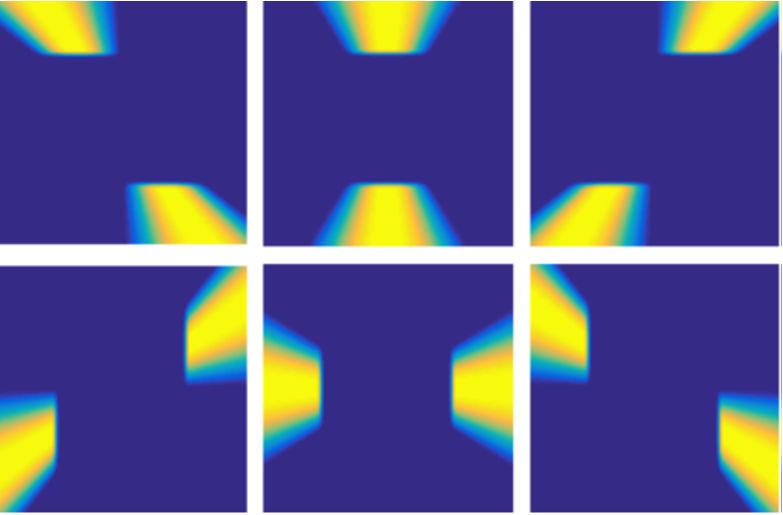
\includegraphics[width=\textwidth]{feasible_mi.pdf}
\end{minipage}
\begin{minipage}[c]{.22\textwidth}
\centering
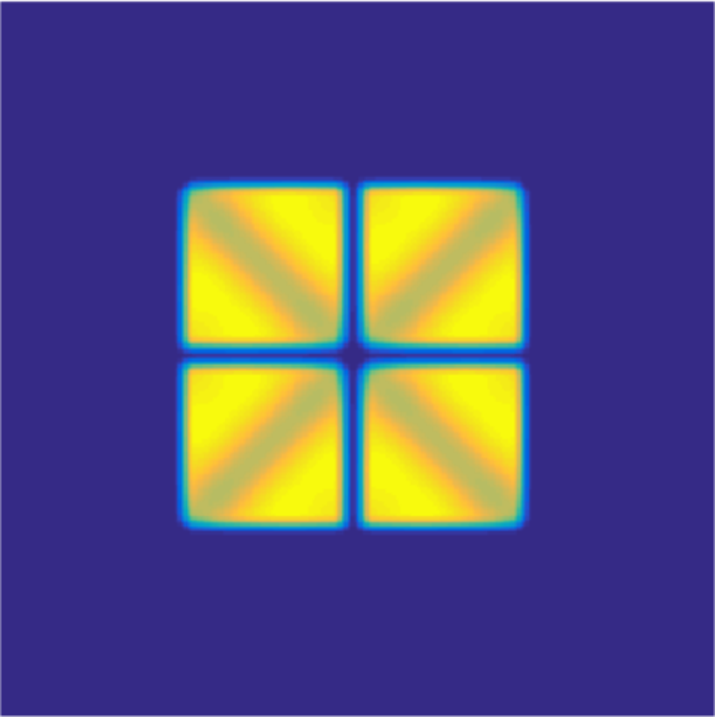
\includegraphics[width=.8\textwidth]{feasible_m0.pdf}
\end{minipage}
\begin{minipage}[c]{.28\textwidth}
\centering
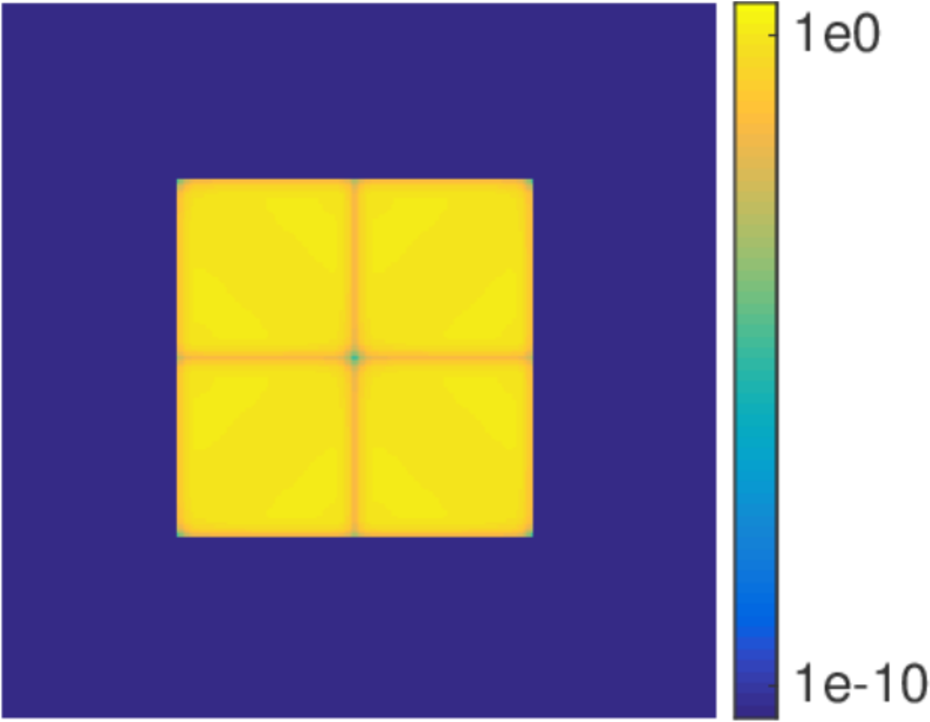
\includegraphics[width=.8\textwidth]{feasible_m0_log.pdf}
\end{minipage}
\caption{Left:  $|\m{i}|$, middle: computed $m_0^C$, right: $\log(m_0^C)$}
\label{fig: tm_i_m_0}
\end{figure}

\subsection{solving $\mc{0}$ and $m_i$}
We compute $\mc{0}$ by solving the following optimization problem similar to \eqref{eq: opt-diff} for the dyadic scheme,
\begin{align}
\min_{\xvec}\; \Vert \V{D}(\mathbf{m}_0^C\circ\xvec)\Vert^2 + \lambda\Vert \wvec\circ\mathbf{m}_0^C\circ\xvec\Vert^2,\quad 
s.t. \; A\xvec = \mathbf{1},\, \mathfrak{D}\xvec = \mathbf{0}
\label{eq: opt-2d}
\end{align}
where $\circ$ is Hadamard product and $\wvec$ is a weight vector and we consider real solution $\xvec$ here.
$A$ in the constraint is the matrix generated from the identity condition \eqref{eq: identity-cond} and $\mathfrak{D}$ is generated from the singularity condition \eqref{eq: singular-cond}. Since $A$ and $\mathfrak{D}$ are linearly independent, \eqref{eq: opt-2d} is feasible. Here, instead of optimizing the properties of $\xvec$ as in \eqref{eq: opt-diff}, we optimize those of $\widetilde{\mathbf{m}_0}^C\circ \xvec$ since $m_0^C \cdot\widetilde{m_0}^C$ will be later re-decomposed into $m_0$ and $\widetilde{m_0}$. In addition, if $m_0^C$ is symmetric with respect to the two coordinates $\omega_x$ and $\omega_y$, then we impose the same symmetry on $\widetilde{m_0}^C$ by solving \eqref{eq: opt-2d} on $[0,\pi)\times[0,\pi)$ and then extend the solution to $[-\pi,\pi)\times[-\pi,\pi)$ by symmetry.

\begin{figure}
\centering
\begin{minipage}[c]{.3\textwidth}
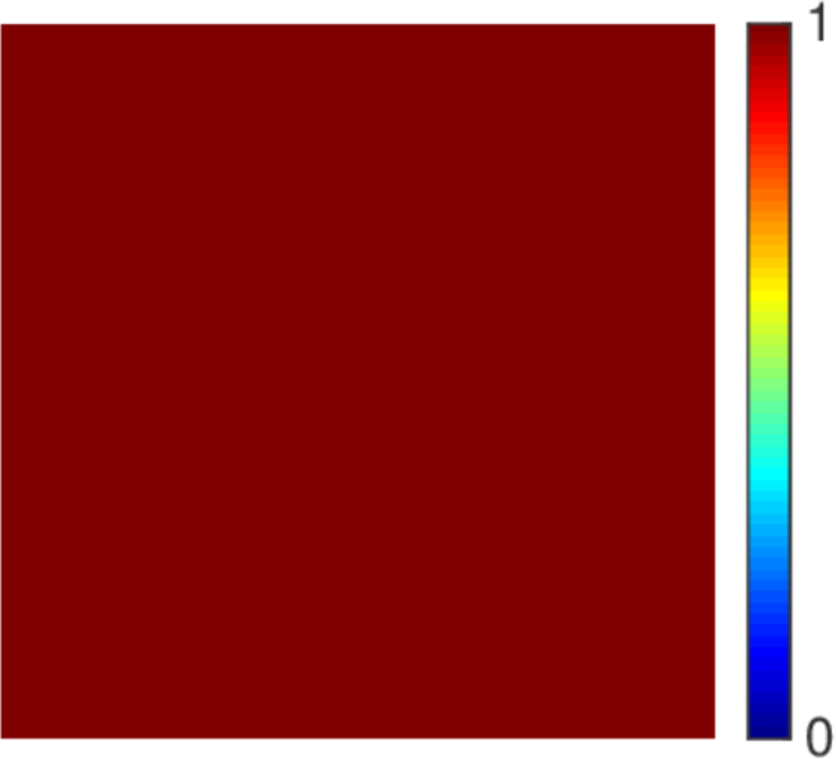
\includegraphics[width = .8\textwidth]{feasible_check.pdf}
\caption{$\vartheta$}\label{fig: feasible}
\end{minipage}
\begin{minipage}[c]{.63\textwidth}%{.28\textwidth}
\centering
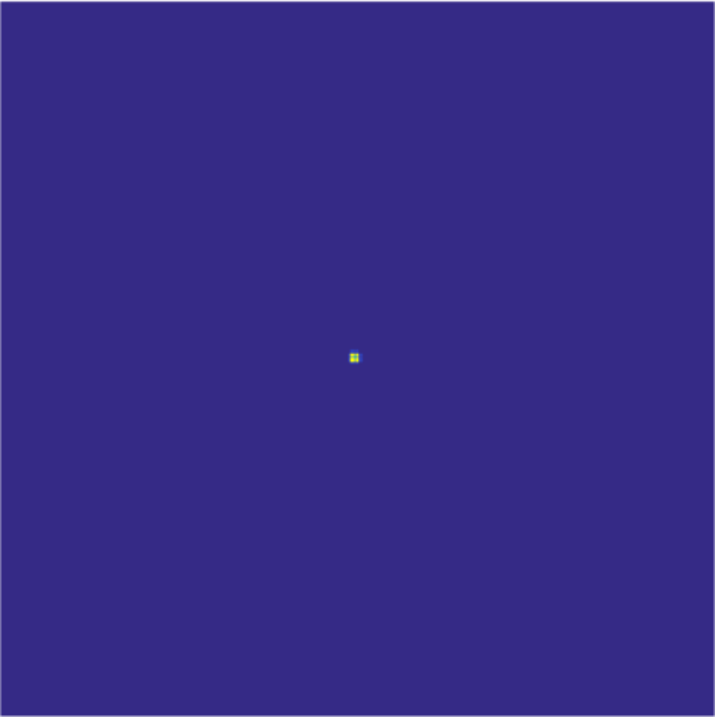
\includegraphics[width = .38\textwidth]{feasible_tm0.pdf}\hspace*{2em}
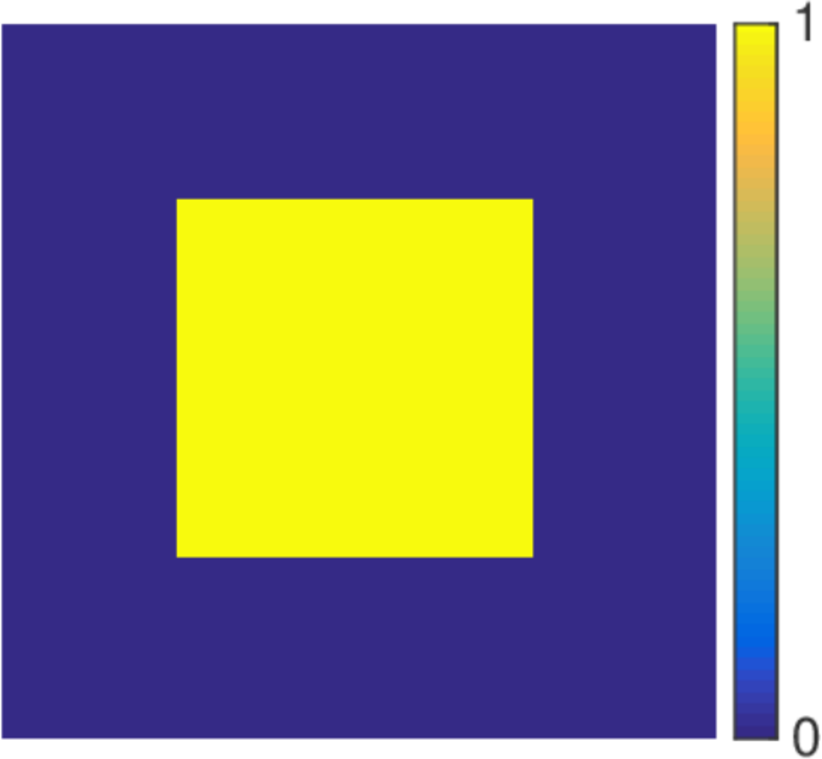
\includegraphics[width = .42\textwidth]{feasible_m0tm0.pdf}
\caption{Left: : computed $\widetilde{m_0}^C$, right: $\widetilde{m_0}^C \cdot m_0^C $}
\label{fig: tm0}
\end{minipage}
\end{figure}

Fig.\ref{fig: tm0} shows $\mc{0}$ obtained from \eqref{eq: opt-2d} and $\widetilde{m_0}^C \cdot m_0^C$ which is $\mathbf{1}_{S_1}$.

In particular, given $\widetilde{m_0}^C \cdot m_0^C = 1$, $\mathbf{b}(\V{\omega}) = \mathbf{0}, \, \forall\,\V{\omega}\in S_1$, hence $\mathbf{m}[2:7] = \mathbf{0}$. 
When $\mathbf{b}(\V{\omega})\neq \mathbf{0}$, \eqref{eq: mi} is a degenerated over-determinant linear system (we also do a sanity check here for the linearity between $\overline{\M}[:,2:7]$ and $\mathbf{b}$ by computing $\vartheta$) and 
$$\mathbf{m}[2:7](\V{\omega}) = \Big(\overline{\M}[:,2:7]\Big)^\dagger\,\mathbf{b}(\V{\omega}),$$
where $\dagger$ is the pseudo-inverse of a matrix. Fig.\ref{fig: m_i} shows the solution $m_i$ of \eqref{eq: mi} and the corresponding spatial filters $\mathcal{F}^{-1}\widetilde{m_0}$.
As shown in Fig.\ref{fig: m_i}, the energy of $m_i$ concentrates on $\{|\omega_x| = \frac{\pi}{2},\, |\omega_y| = \frac{\pi}{2}\}$ where $|\widetilde{m_i}|$ is small, and the filters decay slowly in time domain.

The bi-orthogonal bases constructed is not ideal, despite the regularization on $m_0$ in the optimization \eqref{eq: opt-2d}. Since no explicit regularization is put on $m_i$, it's difficult to control the regularity of the output $m_i$ from the input $\widetilde{m_i}$.

\begin{figure}
\centering
\begin{minipage}[c]{.5\textwidth}
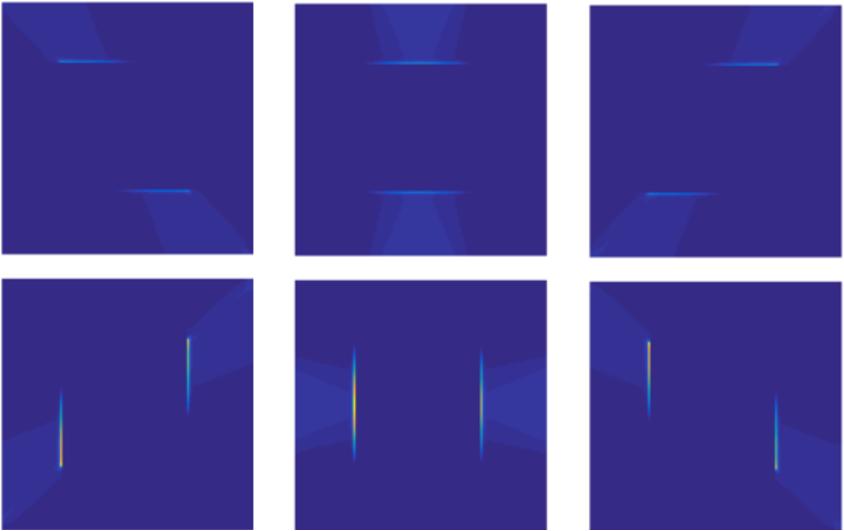
\includegraphics[width = .9\textwidth]{feasible_m.pdf}
\end{minipage}
\begin{minipage}[c]{.48\textwidth}
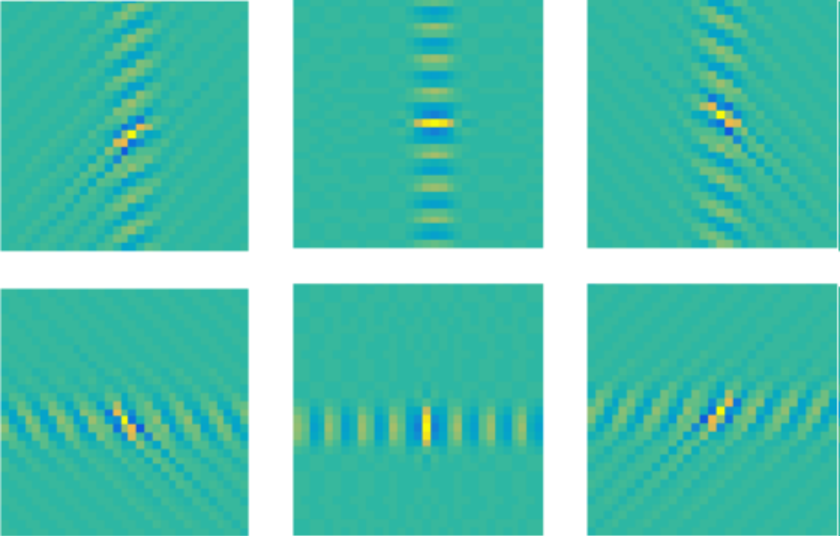
\includegraphics[width = .9\textwidth]{feasible_mi_time.pdf}
\end{minipage}
\caption{Left: $|m_i|,\, i = 1,\cdots,6$, right:$|\mathcal{F}^{-1}m_i|$}
\label{fig: m_i}
\end{figure}
\end{comment}